    \documentclass[dvipsnames]{beamer}
    \usetheme{Madrid}
    \usefonttheme{professionalfonts}
    \usepackage{
        amsmath,
        amssymb,
        fouriernc, % fourier font w/ new century book
        fancyhdr, % page styling
        lastpage, % footer fanciness
        hyperref, % various links
        setspace, % line spacing
        amsthm, % newtheorem and proof environment
        mathtools, % \Aboxed for boxing inside aligns, among others
        float, % Allow [H] figure env alignment
        enumerate, % Allow custom enumerate numbering
        graphicx, % allow includegraphics with more filetypes
        wasysym, % \smiley!
        upgreek, % \upmu for \mum macro
        listings, % writing TrueType fonts and including code prettily
        tikz, % drawing things
        booktabs, % \bottomrule instead of hline apparently
        cancel % can cancel things out!
    }
    \usepackage[
        labelfont=bf, % caption names are labeled in bold
        font=scriptsize % smaller font for captions
    ]{caption}
    \usepackage[font=scriptsize]{subcaption} % subfigures

    \newcommand*{\scinot}[2]{#1\times10^{#2}}
    \newcommand*{\dotp}[2]{\left<#1\,\middle|\,#2\right>}
    \newcommand*{\rd}[2]{\frac{\mathrm{d}#1}{\mathrm{d}#2}}
    \newcommand*{\pd}[2]{\frac{\partial#1}{\partial#2}}
    \newcommand*{\rtd}[2]{\frac{\mathrm{d}^2#1}{\mathrm{d}#2^2}}
    \newcommand*{\ptd}[2]{\frac{\partial^2 #1}{\partial#2^2}}
    \newcommand*{\md}[2]{\frac{\mathrm{D}#1}{\mathrm{D}#2}}
    \newcommand*{\pvec}[1]{\vec{#1}^{\,\prime}}
    \newcommand*{\svec}[1]{\vec{#1}\;\!}
    \newcommand*{\bm}[1]{\boldsymbol{\mathbf{#1}}}
    \newcommand*{\ang}[0]{\;\text{\AA}}
    \newcommand*{\mum}[0]{\;\upmu \mathrm{m}}
    \newcommand*{\at}[1]{\left.#1\right|}

    \let\Re\undefined
    \let\Im\undefined
    \DeclareMathOperator{\Res}{Res}
    \DeclareMathOperator{\Re}{Re}
    \DeclareMathOperator{\Im}{Im}
    \DeclareMathOperator{\Log}{Log}
    \DeclareMathOperator{\Arg}{Arg}
    \DeclareMathOperator{\Tr}{Tr}
    \DeclareMathOperator{\E}{E}
    \DeclareMathOperator{\Var}{Var}
    \DeclareMathOperator*{\argmin}{argmin}
    \DeclareMathOperator*{\argmax}{argmax}
    \DeclareMathOperator{\sgn}{sgn}
    \DeclareMathOperator{\diag}{diag\;}

    \DeclarePairedDelimiter\bra{\langle}{\rvert}
    \DeclarePairedDelimiter\ket{\lvert}{\rangle}
    \DeclarePairedDelimiter\abs{\lvert}{\rvert}
    \DeclarePairedDelimiter\ev{\langle}{\rangle}
    \DeclarePairedDelimiter\p{\lparen}{\rparen}
    \DeclarePairedDelimiter\s{\lbrack}{\rbrack}
    \DeclarePairedDelimiter\z{\lbrace}{\rbrace}

    % \everymath{\displaystyle} % biggify limits of inline sums and integrals
    \tikzstyle{circ} % usage: \node[circ, placement] (label) {text};
        = [draw, circle, fill=white, node distance=3cm, minimum height=2em]
    \definecolor{commentgreen}{rgb}{0,0.6,0}
    \lstset{
        basicstyle=\ttfamily\footnotesize,
        frame=single,
        numbers=left,
        showstringspaces=false,
        keywordstyle=\color{blue},
        stringstyle=\color{purple},
        commentstyle=\color{commentgreen},
        morecomment=[l][\color{magenta}]{\#}
    }

\begin{document}

\begin{frame}
    \frametitle{Review}

    \begin{itemize}
        \item Last time: found flux absorbed $\neq$ flux injected w/
            $\nu$-extrapolation, \textbf{must have reflection.}

        \item Hypothesis:
            \begin{equation}
                \vec{u} = A_0\vec{u}_0 + \delta \vec{u},
            \end{equation}
            where $A_0$ is set by forcing, $\delta \vec{u}$ is ``turbulent.''

        \item Since $S_{px} = \ev*{\rho u_xu_z}_x$, decided to plot
            \begin{equation}
                \delta S_{px} = \ev*{\rho \delta u_x \delta u_z}_x.
            \end{equation}
    \end{itemize}
\end{frame}

\begin{frame}
    \frametitle{Results}
    \framesubtitle{Driving amplitude}

    \begin{itemize}
        \item Actually, discovered $A < A_0$, \textbf{driving amplitude changes
            over time} (via convolution). Oscillation timescale $\sim
            \frac{z_0 - z_c}{v_{gz}}$ for higher order modes.

        \item Adjusting for this gives $\ev*{\rho u_{x0} \delta u_z}_x,
            \ev*{\rho \delta u_x u_{z0}}_x$ centered on zero, no net flux.

        \begin{figure}[t]
            \centering
            \begin{subfigure}{0.45\textwidth}
                \centering
                \includegraphics[width=\textwidth]{../../sims/2d_3_final/snapshots_lin_1/f_amps.png}
                \caption{Linear excited $\frac{u_x}{u_{x0}}, \frac{u_z}{u_{z0}}$ over
                time.}
            \end{subfigure}
            \begin{subfigure}{0.45\textwidth}
                \centering
                \includegraphics[width=\textwidth]{../../sims/2d_3_final/snapshots_nl_4/f_amps.png}
                \caption{Nonlinear excited $\frac{u_x}{u_{x0}}, \frac{u_z}{u_{z0}}$ over
                time.}
            \end{subfigure}
        \end{figure}
    \end{itemize}
\end{frame}

\begin{frame}
    \frametitle{Results}
    \framesubtitle{Driving Amplitude}

    \begin{figure}[t]
        \centering
        \includegraphics[width=0.6\textwidth]{../../sims/2d_3_final/snapshots_nl_4/fluxes_time.png}
        \caption{Decompositions of the flux over time. $01$ means $u_{x0} \delta
        u_z$. Oscillating $01, 10$ implies reflected $k_z \to -k_z$ mode.}
    \end{figure}
\end{frame}

\begin{frame}
    \frametitle{Results}
    \framesubtitle{Front Position}

    \begin{figure}[t]
        \centering
        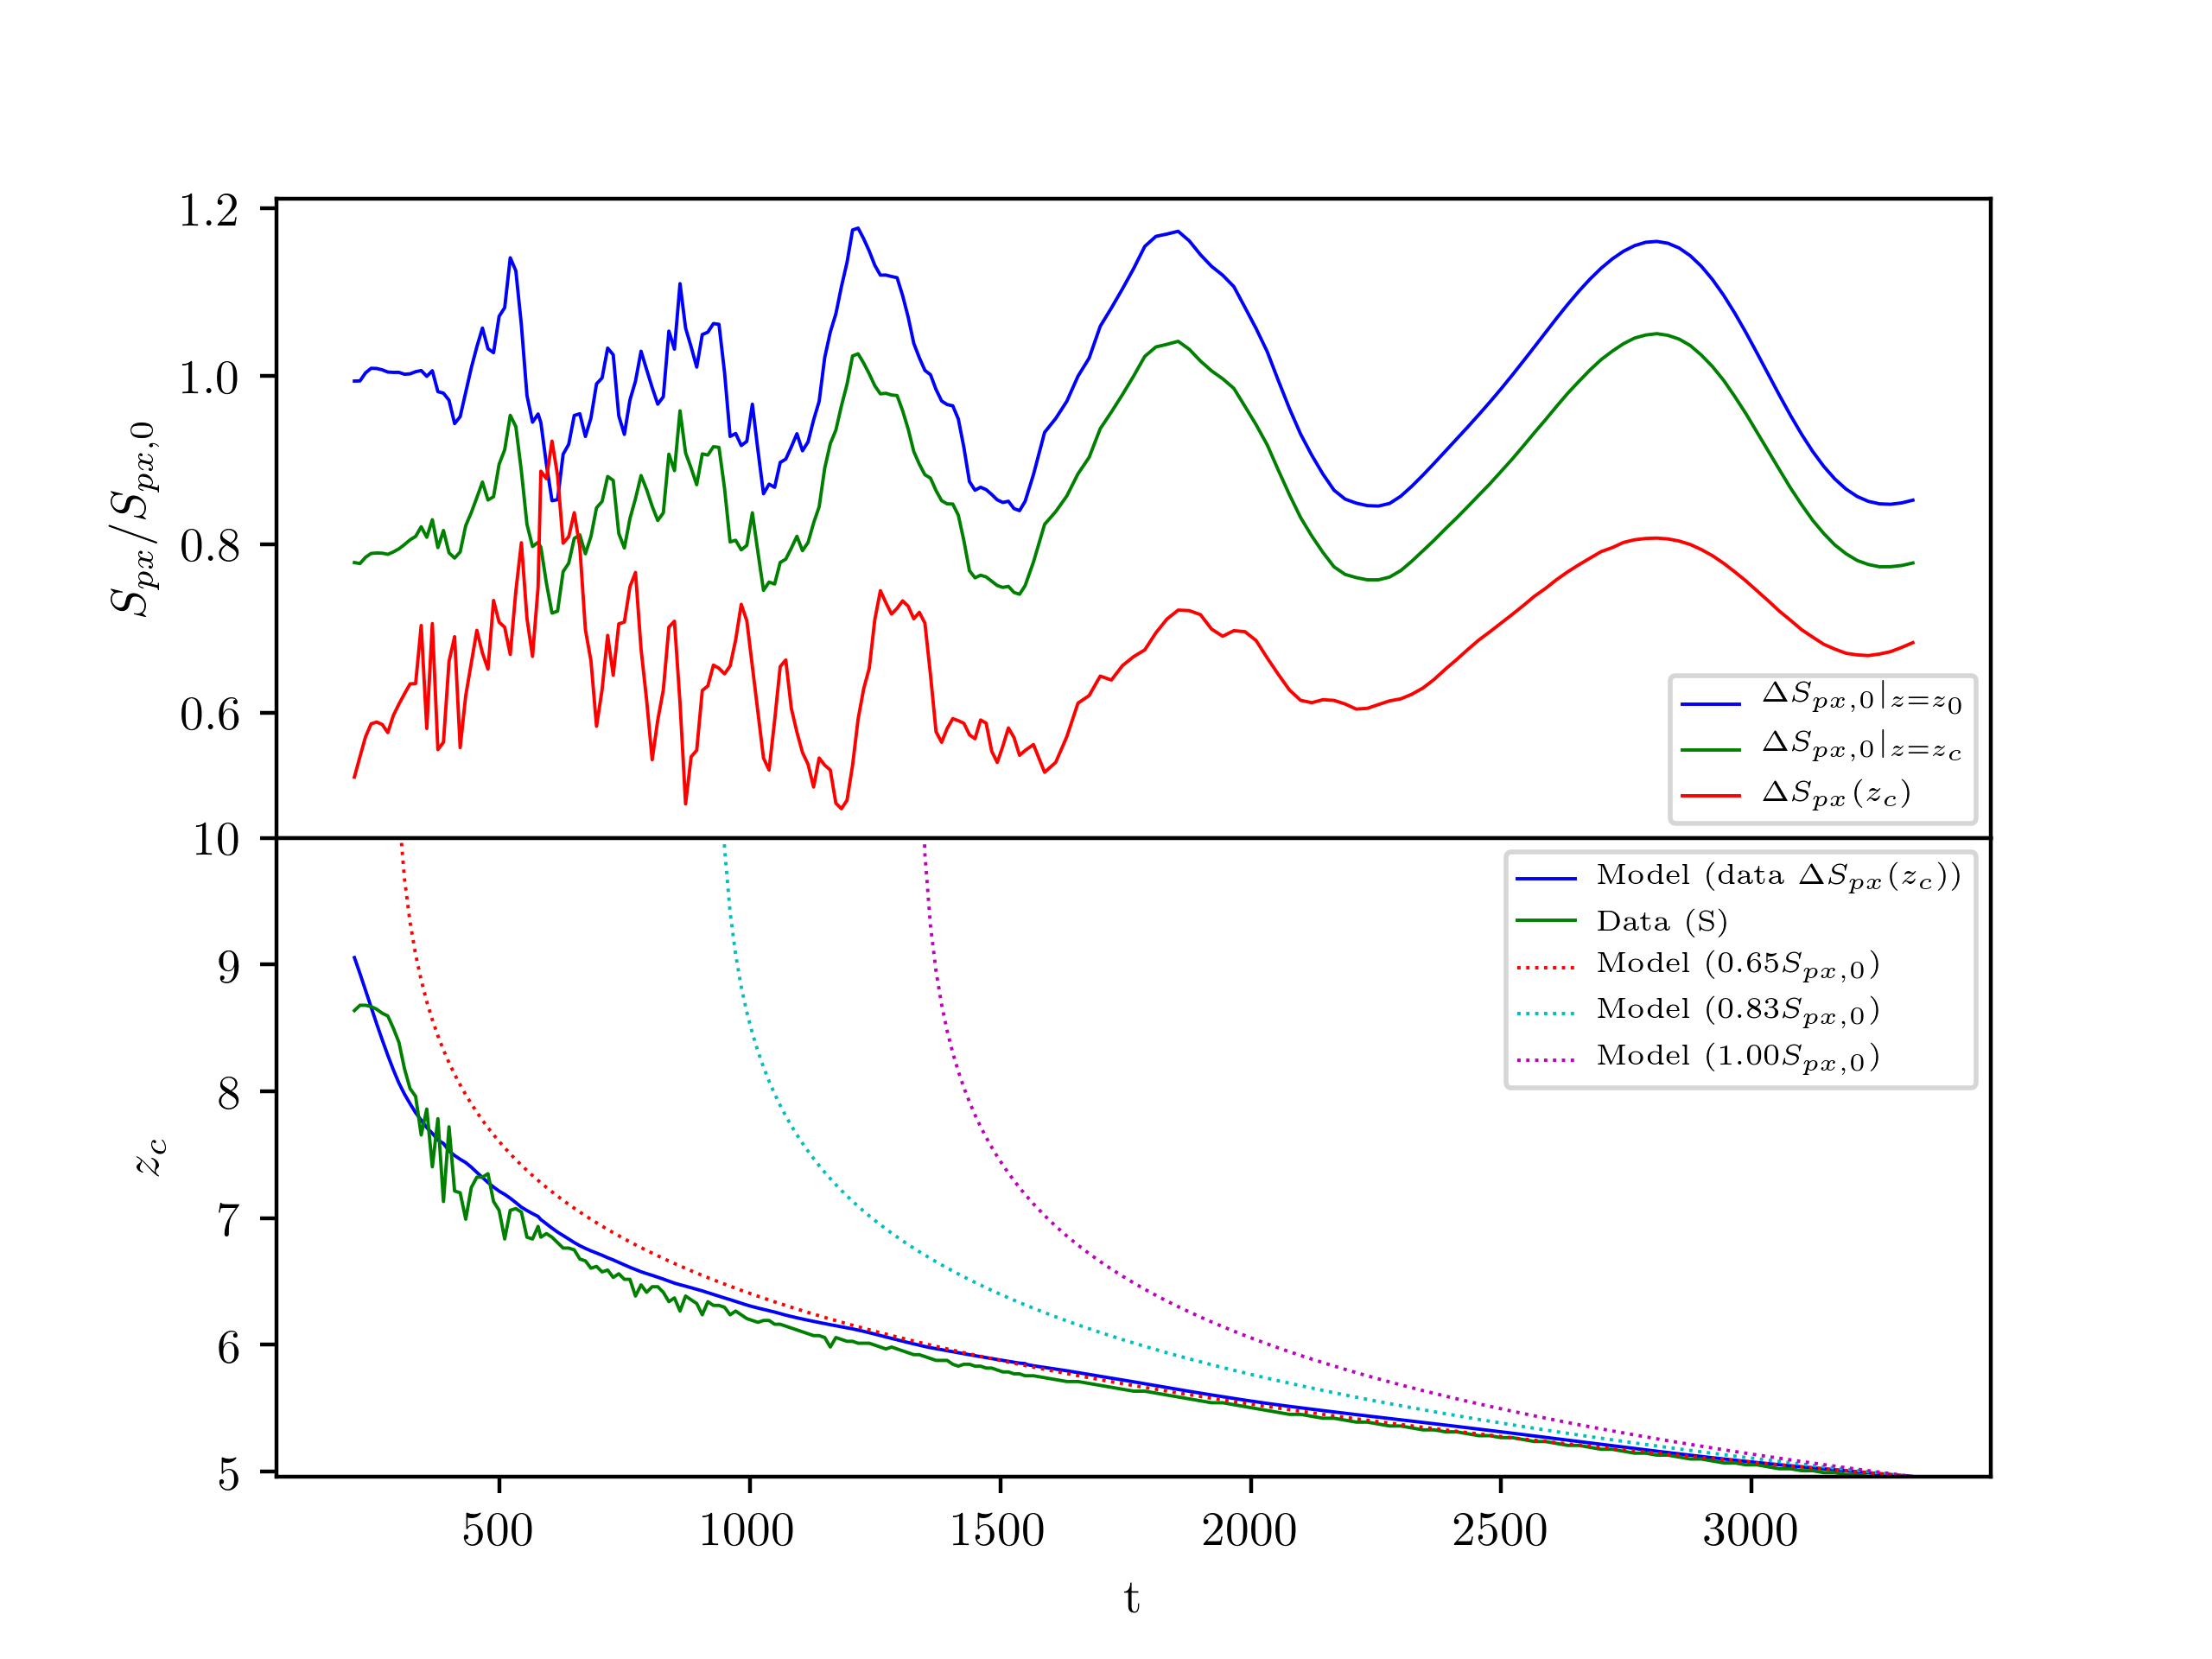
\includegraphics[width=0.6\textwidth]{../../sims/2d_3_final/snapshots_nl_4/front.png}
        \caption{Front evolution, nonlinear.}
    \end{figure}
\end{frame}

\begin{frame}
    \frametitle{Results}
    \framesubtitle{Minimum Ri}

    \begin{figure}[t]
        \centering
        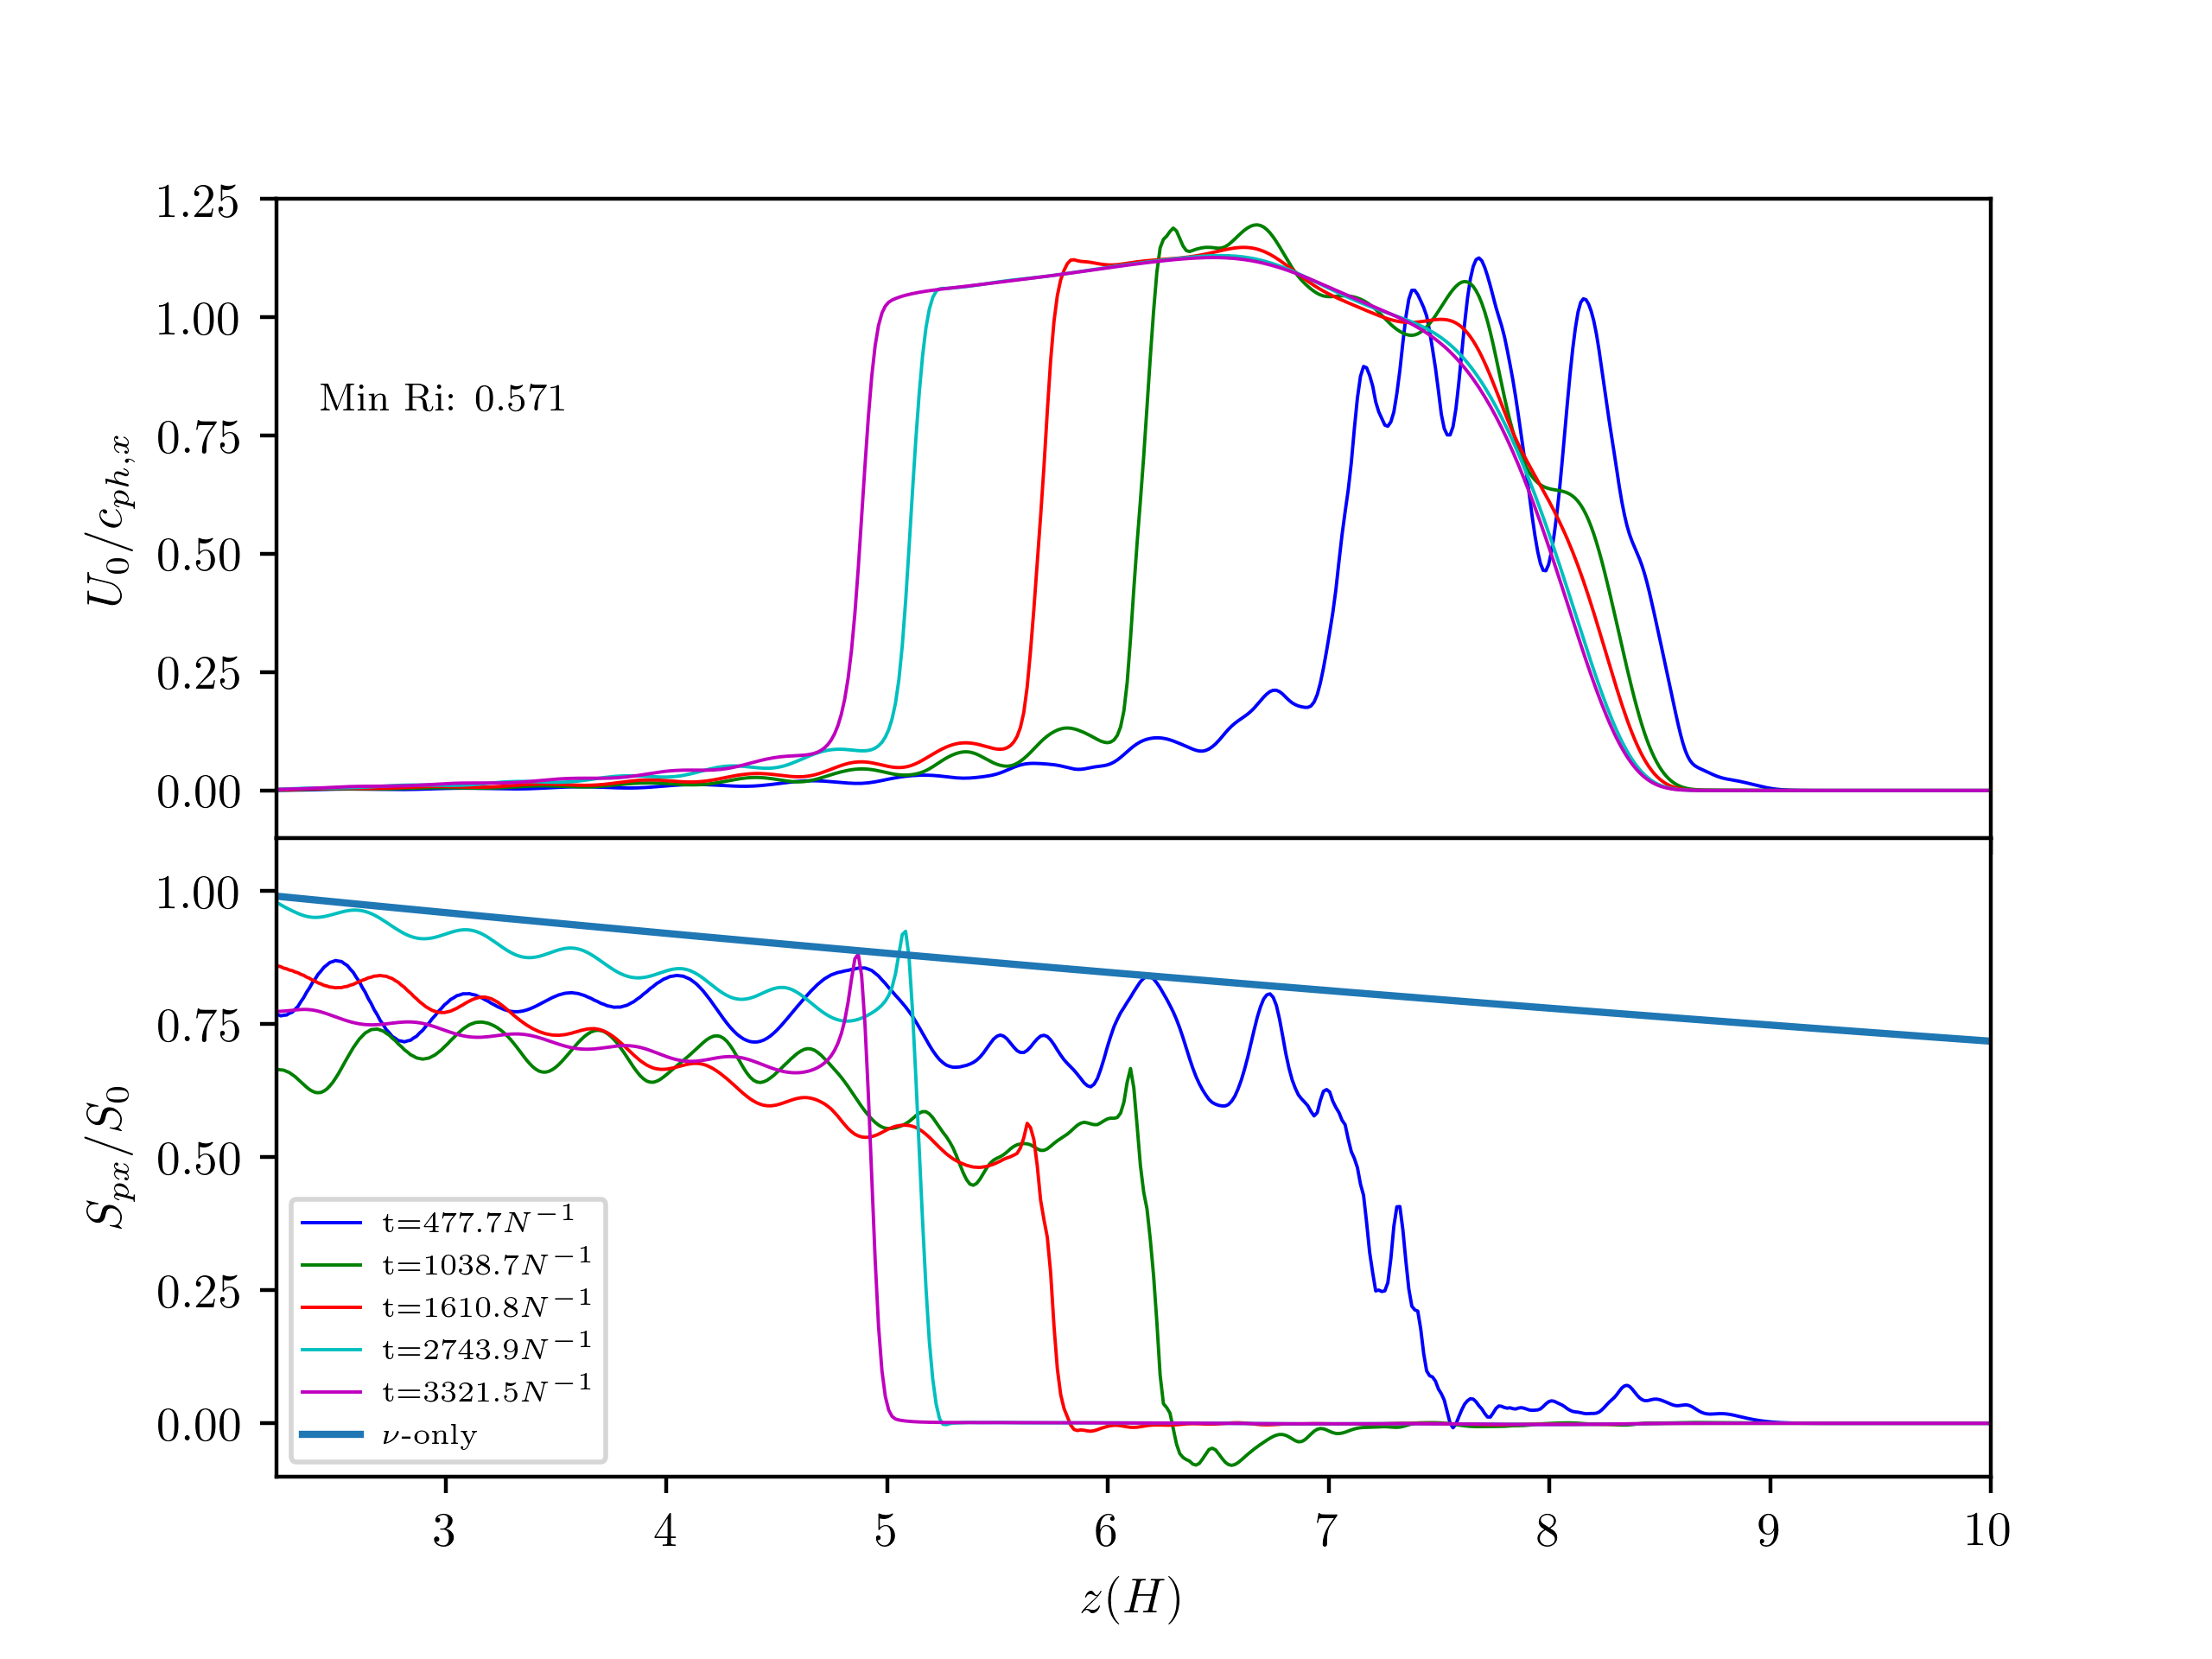
\includegraphics[width=0.6\textwidth]{../../sims/2d_3_final/snapshots_nl_4/fluxes.png}
        \caption{Mean flow and flux evolution, non-linear.}
    \end{figure}
\end{frame}

\begin{frame}
    \frametitle{Conclusion}
    \framesubtitle{All effects}

    \begin{itemize}
        \item Excite wave with $S_{px}$. Deposit some $\eta S_{px}$ in
            critical layer (efficiency $\eta$).

        \item Critical layer width $\delta z$ such that $\mathrm{Ri} \gtrsim
            \frac{1}{4}$.

        \item Critical layer position obeys $\rho c_{ph, x} \pd{z_c}{t}
            = -\eta S_{px}$, or ($\tau = \frac{H\rho_0(z = 0)c_{ph,x}}
            {\eta S_{px}}$)
            \begin{equation}
                z_c(t) = -H\ln \frac{t - t_i + \tau e^{-z_i/H}}{\tau},
            \end{equation}

        \item Reflect $(1 - \eta)S_{px}$, some in $k_z \to k_z$ linear
            reflection, some in higher-order modes.

        \item Reflected wave causes inefficient excitation $S_{px,0} \to \alpha
            S_{px, 0}$, $\alpha \lesssim 1$.

        \item Probably can't be any more exact, time delays + noisy data.
    \end{itemize}
\end{frame}

\end{document}

